\section{Experimental Evaluation}
\label{sec:evaluation}

This evaluation demonstrates that \algname outperforms previous approaches and achieves competitive results compared to state-of-the-art implementations, with performance gains depending on the convolution parameters.
In end-to-end models, \algname improves inference execution time by up to 1.47$\times$. \rsec{standalone-conv} discusses standalone layer performance and \rsec{end-to-end} discusses end-to-end model inference.

\subsection{Setup}
\label{sec:setup}

\begin{table*}
    \centering
    \begin{minipage}{0.3\linewidth}
        \caption{Experimental configuration}
        \label{tab:specs}
        \small
        \centering
        \begin{tabular}{l|l}
        CPU              & i7-14700K       \\ \hline
        Cores Used       & 8 P-Cores       \\ \hline
        Frequency        & \SI{3}{GHz} (locked) \\ \hline
        Memory           & \SI{64}{GiB} DDR5
        \end{tabular}
    \end{minipage}
    \hfill
    \begin{minipage}{0.28\linewidth}
        \caption{Software versions}
        \label{tab:version}
        \small
        \centering
        \begin{tabular}{l|l}
        PyTorch          & 2.5.1     \\ \hline
        OneDNN           & 3.5.3     \\ \hline
        OneMKL           & 2025.0.0  \\ \hline
        BLIS             & 1.0
        \end{tabular}
    \end{minipage}
      \begin{minipage}{0.40\linewidth}
        \caption{Models and convolutional layers}
        \label{tab:models}
        \small
        \centering
        \begin{tabular}{l|c|c|}
                             & TorchVision & Timm \\ \hline
        Models               & 98          & 1149 \\
        Unique \emph{Conv2D} & \multicolumn{2}{c|}{9826} \\
        \end{tabular}
    \end{minipage}
\end{table*}

\rtab{specs} provides details of the experimental machine configuration.
Experiments run on performance (P) cores, and multithread runs use all 8 P-cores; the governor is set to \emph{performance}, frequency locked at 3 GHz, and Hyper-Threading and Turbo Boost are disabled.
The system runs Ubuntu 22.04.5 with kernel 6.5.0.
\rtab{version} lists the software versions used, with additional details available in the accompanying artifact. % TODO

Two collections of vision models are used: \emph{TorchVision}~\cite{torchvision} and \emph{Timm}~\cite{timm}, both of which provide models for PyTorch, including architectures such as MobileNet~\cite{MobilenetV3}, ResNet~\cite{resnet2016}, and EfficientNet~\cite{efficientnet2019}.
\rtab{models} summarizes the number of unique models in each collection and the distinct convolution layers they contain.
TorchVision models that do not take images as input (video and optical flow models) are not included in \rtab{models}, and quantized models are omitted because they do not use PyTorch's standard \emph{Conv2D} implementation.

\subsection{Standalone Convolutions}
\label{sec:standalone-conv}

\begin{table}[t]
    \caption{Tensor layouts used by evaluated methods.}
    \label{tab:standalone-conv-layout}
    \small
    \centering
    \begin{tabular}{l|c|c}
                       & Image/Output Layout        & Weight Layout  \\ \hline
    Im2col             & \texttt{N,C,H,W} & \texttt{OC,IC,FH,FW}  \\ \hline
    Yaconv &
      \multirow{3}{*}{\texttt{N,H,W,C}} &
      \multirow{3}{*}{\texttt{FH,FW,IC,OC}} \\
    \algname           &                     &                      \\
    LibTorch-\algname  &                     &                      \\ \hline 
    LibTorch           & \texttt{N,H,W,C} & \texttt{OC,FH,FW,IC}
    \end{tabular}
\end{table}

This experiment evaluates \algname by measuring the execution time of the standalone convolutional layers from \rtab{models}.
The evaluated convolution methods are listed below and \rtab{standalone-conv-layout} summarizes the input image, weight, and output layouts they use.
Conversion to these layouts is not included in the execution time measurements.
For methods that rely on GEMM calls, Intel's OneMKL is used as the default BLAS library.
Before measuring performance, the correctness of these methods was verified using LibTorch as the reference output. 

\begin{enumerate}
    \item \textbf{Yaconv}, a convolution method introduced by \citet{Korostelev2023} as an extension of the BLIS library.
    It uses the author's original implementation, with modifications to prevent runtime errors and to remove extra generated elements that are not part of the output.
    
    \item \textbf{Im2col}, a C implementation based on the Caffe framework that transforms convolution into GEMM operations through the Im2col data transformation~\cite{chellapilla2006, caffe2014}.
    Parallelism is handled by the GEMM library.
    
    \item \textbf{\algname}, a C implementation of \algfullname that leverages OpenMP for parallelism. It also utilizes OneMKL's JIT optimization for small GEMM sizes, which is handled automatically by the library.

    \item \textbf{LibTorch}, PyTorch's C++ API of \emph{Conv2D}, which is used when running models with convolutional layers.
    It may call multiple convolution backends, including OneDNN.
    OneDNN supports multiple convolution algorithms, but in LibTorch, it is set to use direct convolution implementations.
    LibTorch also allocates its output tensor as part of the computation.

    \item \textbf{LibTorch-\algname}, the \algname algorithm integrated into PyTorch, similar to \textbf{LibTorch}, also allocates the output tensor.
  \end{enumerate}

The experiment runs convolutions with a custom benchmark based on Google Benchmark~\cite{googlebench} and ConvBench~\cite{convbench}. 
Methods run layers in random order; each configuration runs at least ten times (or until 0.5 seconds) with a 0.1 second warm-up, and the mean over five or more repeats is reported.
Additional repetitions are done when 95\% confidence intervals (CI) overlaps between two compared points and differences exceeded 1\%.
If the CI overlaps and the difference is less than 1\%, the comparison is considered insignificant.

In the following comparison graphs (\rfig{single-conv-comparison}), the bars represent the speedup of one method over another across different convolution layers. 
The legend indicates the number of speedup and slowdown cases, while the x-axis label specifies the total number of layers shown.
The y-axis uses a logarithmic scale to accommodate the wide range of values.
Unlike traditional speedup graphs, which restrict slowdown values between 1 and 0, both speedup and slowdown are unbounded and symmetrical.
The bars are sorted by speedup.
Speedup values are clipped at the 0.99 quantile, with the maximum value displayed at the top of the graph.
Similarly, slowdown values are clipped at the 0.01 quantile, with the minimum value shown at the bottom of the graph.

The total number of layers shown on the x-axis may differ from the total in \rtab{models} due to omitted layers.
Two conditions lead to the omission of a layer:
Layers where the execution time difference is insignificant, and layers filtered by a heuristic because executing them with the new method is not beneficial.
The caption of \rfig{single-conv-comparison} specifies heuristic-based exclusions.

A heuristic applied in all comparisons is the exclusion of pointwise layers (6072 layers from the total in \rtab{models}).
This is because pointwise convolutions can be computed directly as GEMM without additional transformations (\eg, Im2col).
\algname is designed to extract multiple smaller GEMMs within convolutions that require the Im2col data layout transformation.
Direct GEMM, when applicable, is a simpler and more efficient approach.

Furthermore, six representative convolution layers, described in \rtab{perf-layers}, are used to illustrate the memory hierarchy effects of the compared methods.
Layers 1 to 3 are more conventional convolution configurations with decreasing input height and width.
Layer 4 is a strided convolution that does not overlap image patches.
Layer 5 is a grouped (depthwise) convolution, and Layer 6 represents a dilated convolution.
For the tables with memory metrics in this section, results were collected using the Linux Perf tool~\cite{Perf}.
The methodology for Perf runs was adjusted so that all compared methods execute the same number of iterations, with a minimum of one hundred iterations.
Reported Perf events are the average of one hundred such runs, which were run on a single thread for better measurement accuracy.

% Layer 1: 1 32 112 112 64 3 3 1 1 1 1 1 1 1 1 1 0 0
% Layer 2: 1 64 56 56 64 3 3 1 1 1 1 1 1 1 1 1 0 0
% Layer 3: 1 224 7 7 224 3 3 1 1 1 1 1 1 1 1 1 0 0
% Layer 4: 1 320 14 14 320 2 2 0 0 0 0 2 2 1 1 1 0 1
% Layer 5: 1 384 14 14 384 3 3 1 1 1 1 1 1 1 1 384 0 1
% Layer 6: 1 960 33 33 256 3 3 12 12 12 12 1 1 12 12 1 0 0

\begin{table}[t]
    \caption{Parameters for convolution layers used in memory hierarchy metrics comparison. Batch is set to 1.}
    \label{tab:perf-layers}
    \footnotesize
    \setlength{\tabcolsep}{3pt}
    \centering
    \begin{tabular*}{\columnwidth}{@{\extracolsep{\fill}} r r r r r r r r r r r}
          & \texttt{IC}  & \texttt{IH}  & \texttt{IW}  & \texttt{OC}  & \texttt{FH},\texttt{FW} & \texttt{PH},\texttt{PW} & \texttt{SH},\texttt{SW} & \texttt{DH},\texttt{DW} & \texttt{GR} \\ \hline
    \#1   & 32  & 112 & 112 & 64  & 3,3   & 1,1   & 1,1   & 1,1   & 1   \\
    \#2   & 64  & 56  & 56  & 64  & 3,3   & 1,1   & 1,1   & 1,1   & 1   \\
    \#3   & 224 & 7   & 7   & 224 & 3,3   & 1,1   & 1,1   & 1,1   & 1   \\
    \#4   & 320 & 14  & 14  & 320 & 2,2   & 0,0   & 2,2   & 1,1   & 1   \\
    \#5   & 384 & 14  & 14  & 384 & 3,3   & 1,1   & 1,1   & 1,1   & 384 \\
    \#6   & 960 & 33  & 33  & 256 & 3,3   & 12,12 & 1,1   & 12,12 & 1   \\
    \end{tabular*}
\end{table}

\begin{figure*}[t]
  \centering

  % Row 1
  \begin{subfigure}{0.32\linewidth}
      \centering
      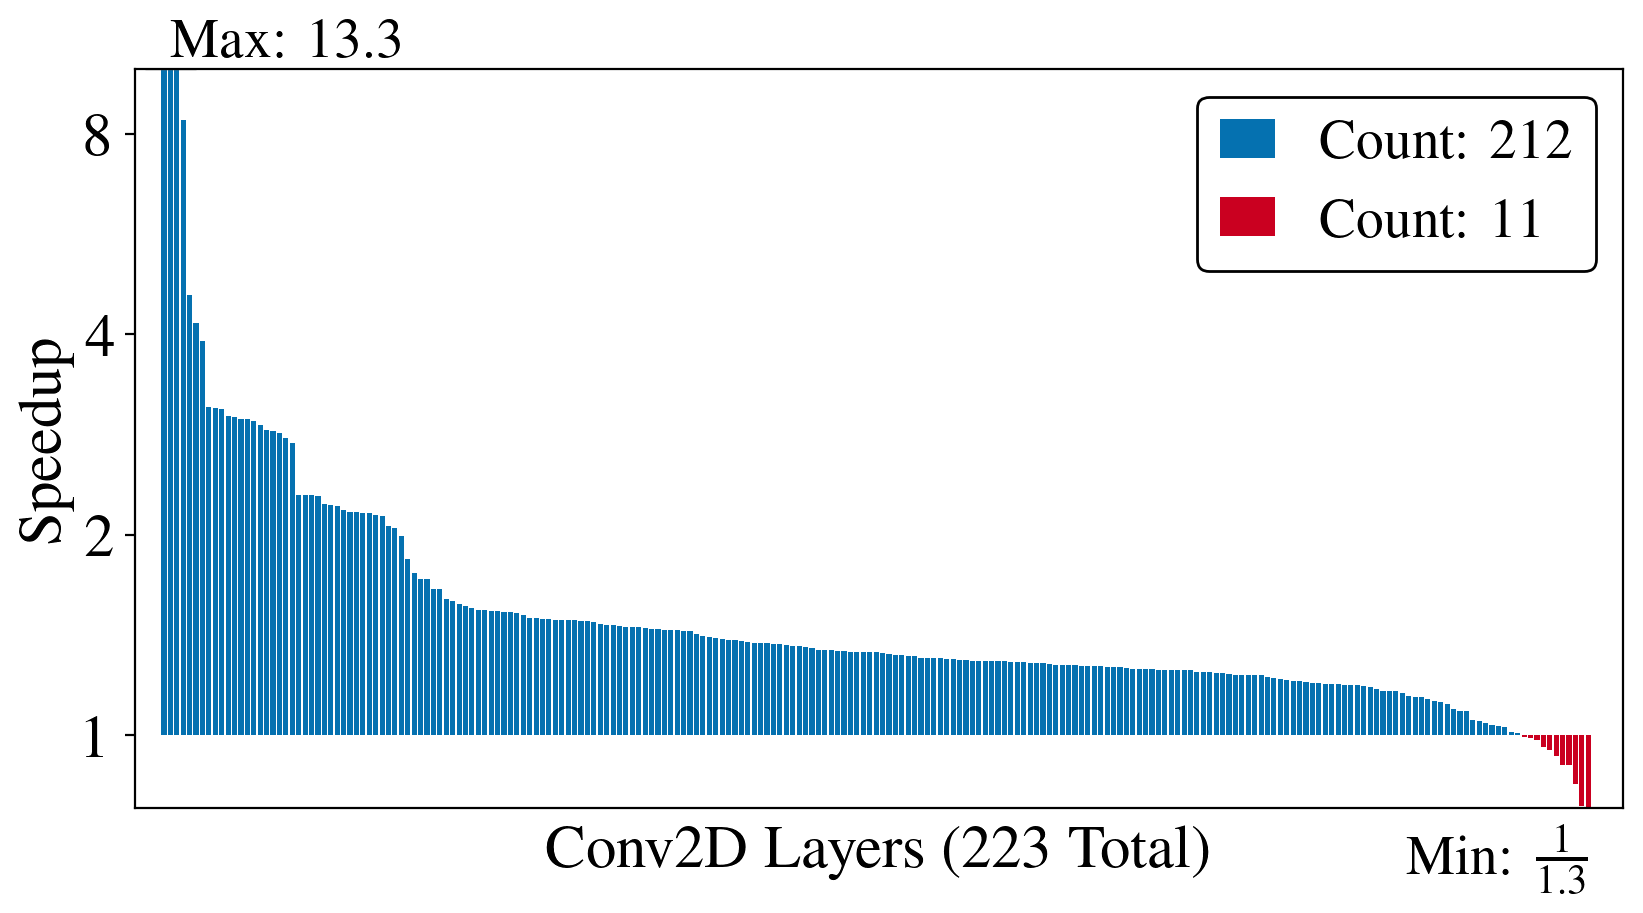
\includegraphics[width=\linewidth]{figures/yaconv-zconv-blis.png}
      \caption{\algname (BLIS as BLAS) over \textbf{Yaconv}}
      \label{fig:yaconv-comparison-blis}
  \end{subfigure}
  \hfill
  \begin{subfigure}{0.32\linewidth}
      \centering
      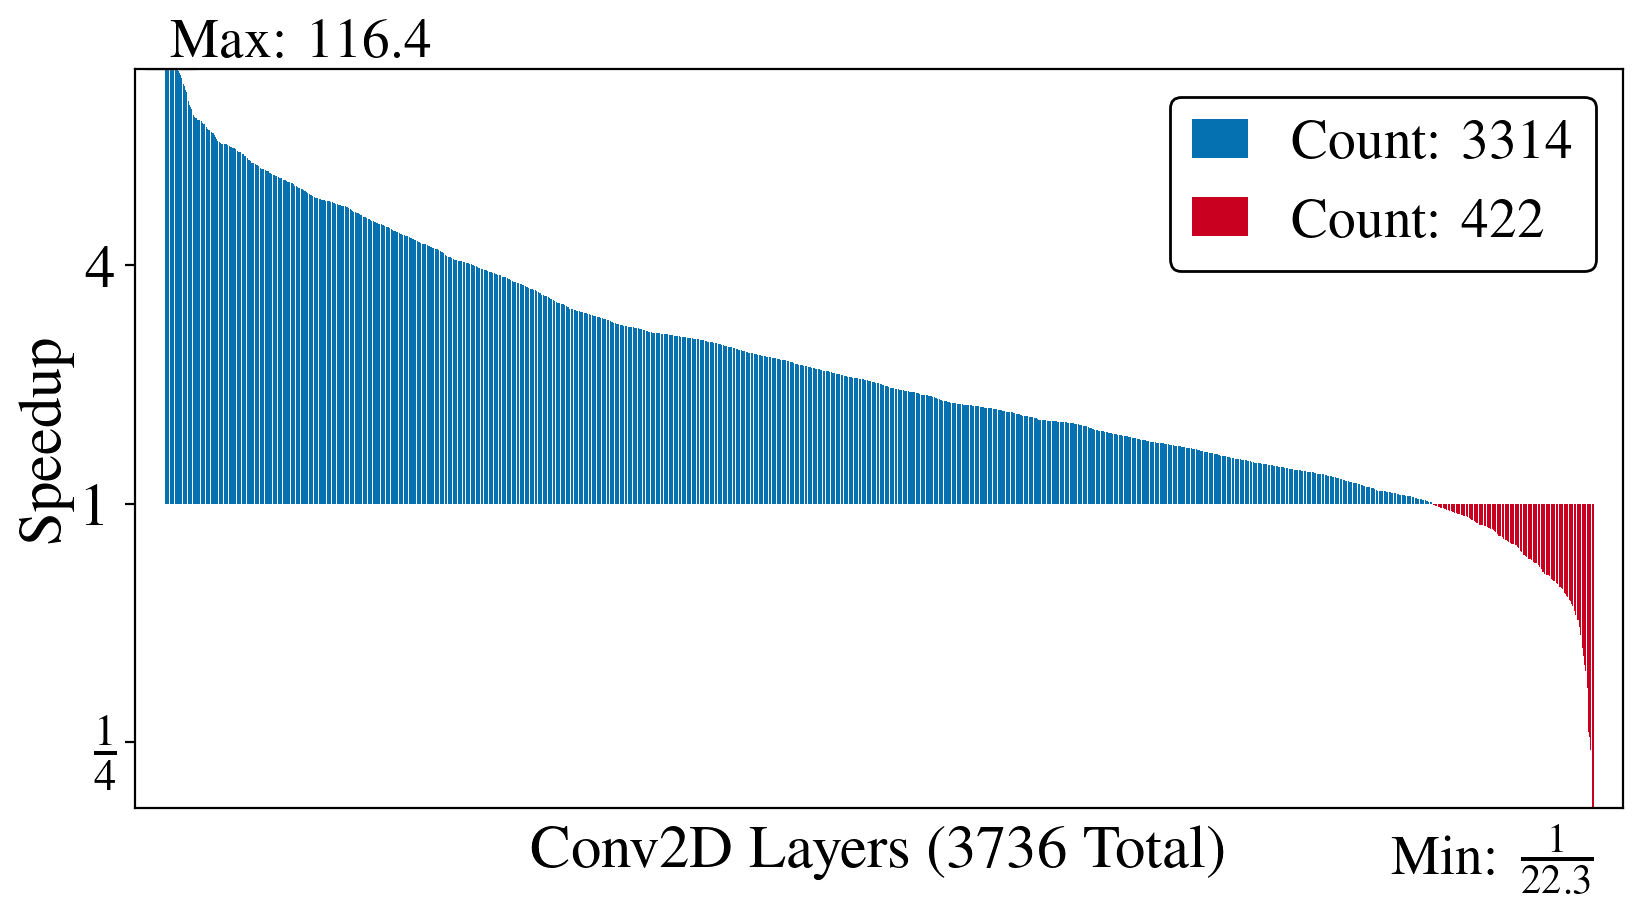
\includegraphics[width=\linewidth]{figures/im2col-multithread.png}
      \caption{\algname over \textbf{Im2col}}
      \label{fig:im2col-comparison-multi}
  \end{subfigure}
  \hfill
  \begin{subfigure}{0.32\linewidth}
      \centering
      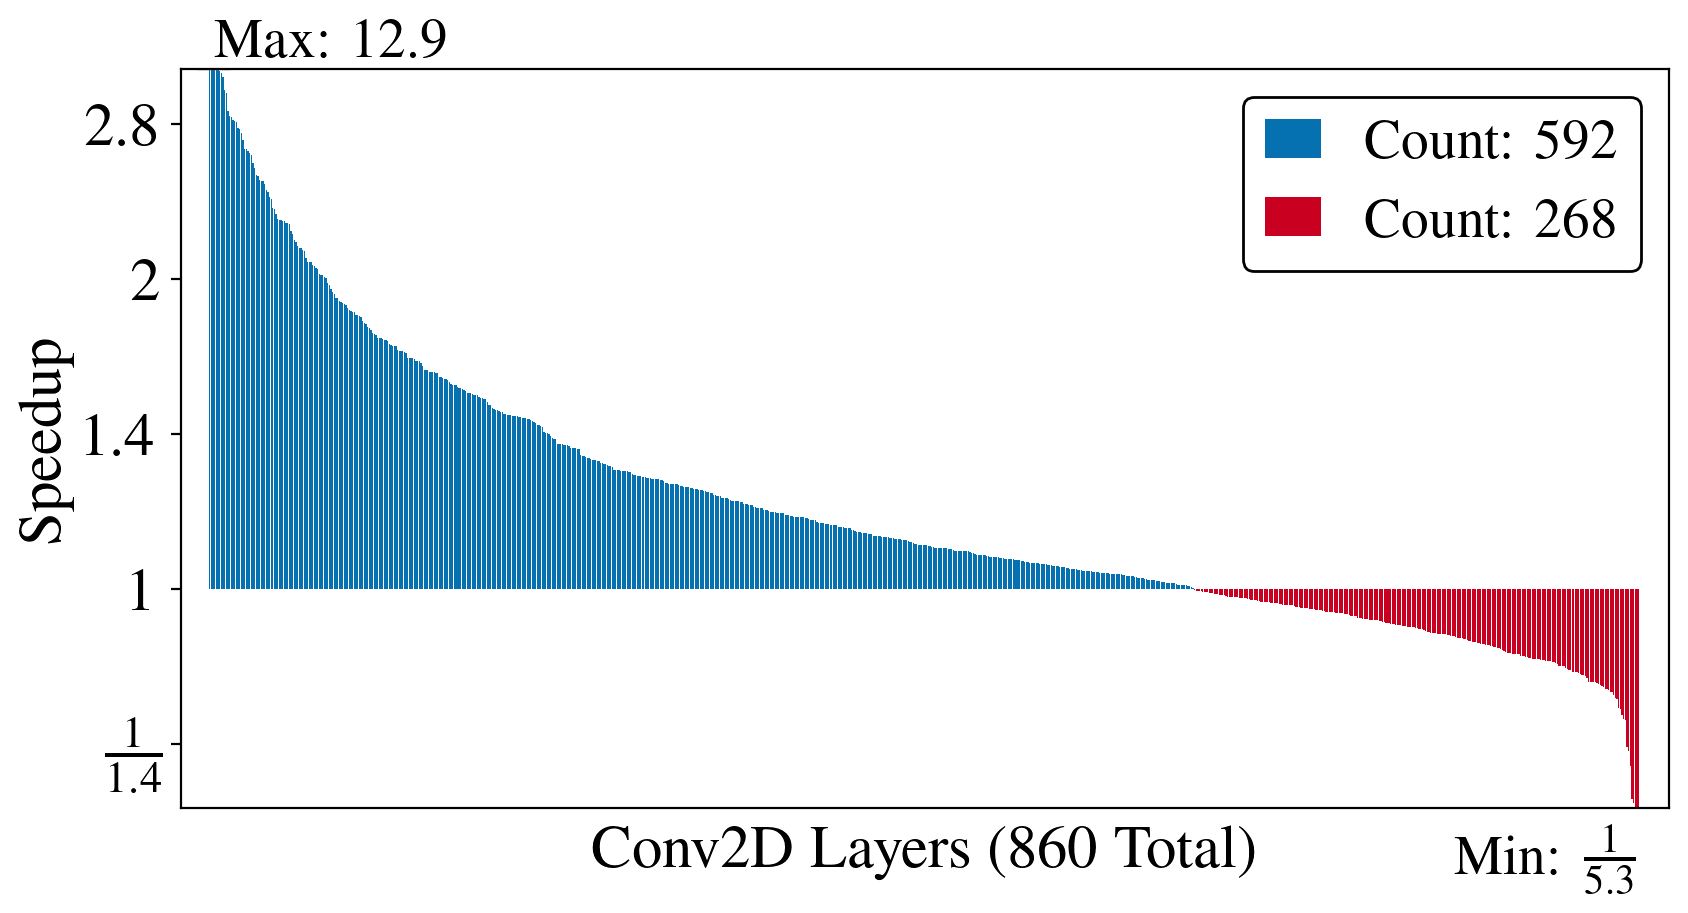
\includegraphics[width=\linewidth]{figures/libtorch-multithread.png}
      \caption{LibTorch-\algname over \textbf{LibTorch}}
      \label{fig:libtorch-comparison-multi}
  \end{subfigure}

  \caption{Improvement of \algname over multiple convolution algorithms on individual \emph{Conv2D} layers. All graphs exclude pointwise layers. Yaconv graphs exclude layers that are unsupported by Yaconv, and for which Yaconv generated incorrect results. The LibTorch graph excludes grouped layers and follows a heuristic defined in \rsec{libtorch}. Executions are multithreaded, except for the Yaconv comparison.}
  \label{fig:single-conv-comparison}
\end{figure*}

\subsubsection{Yaconv}
\label{sec:eval:yaconv}

Figure~\ref{fig:yaconv-comparison-blis} compares \algname against Yaconv.
For this comparison, \algname is executed with a single thread because Yaconv does not support multithreading.
Yaconv does not handle strided, dilated, or grouped convolutions; additionally, out of the 6369 \emph{Conv2D} layers supported by Yaconv, 425 had incorrect results.
These layers were excluded from the comparison.
As Yaconv is integrated into the BLIS library, \algname also utilizes BLIS as its BLAS provider for an accurate comparison of both methods.
The results show significant improvements across almost all \emph{Conv2D} layers, with a maximum speedup of 13$\times$.
\rtab{yaconv-perf} compares memory hierarchy metrics for the two layers from \rtab{perf-layers}, which are supported by Yaconv.
Bolded values highlight metrics improved by \algname.

\begin{table}[t]
    \caption{Metrics of \textbf{Yaconv / ZConv using BLIS} as BLAS}
    \label{tab:yaconv-perf}
    \small
    \setlength{\tabcolsep}{4pt} % reduce column spacing
    \centering
    \begin{tabular}{c|cc|cccc|c}
        & \multicolumn{2}{c|}{Execution} & \multicolumn{4}{c|}{Load Misses} & \multirow{2}{*}{Page Faults} \\
        Layer & Time & Instr. & L1 & L2 & L3 & dTLB & \\ \hline
        1 & \textbf{1.3} & \textbf{1.3} & 0.8 & \textbf{8.4} & \textbf{16.6} & \textbf{77.5} & \textbf{278.0} \\
        2 & \textbf{1.3} & \textbf{1.3} & 0.2 & \textbf{17.2} & \textbf{26.4} & \textbf{70.4} & \textbf{345.6} \\
    \end{tabular}
\end{table}

Three main factors contribute to these improvements.
\begin{enumerate*}[label=(\arabic*)]
\item Due to its packing decisions, Yaconv performs additional computations that introduce extraneous elements in its output, requiring a temporary buffer to filter them out.
In contrast, \algname does not perform unnecessary computations.
This factor is evidenced by \algname executing fewer instructions, even though both algorithms have a similar design.
%
\item All optimizations (\eg, loop ordering) in Yaconv, besides the GEMM microkernel, are manually implemented.
\algname delegates most of these optimizations to the GEMM kernel, benefiting from its more advanced and flexible optimization strategies.
%
\item Lastly, Yaconv is tightly integrated with the BLIS library, whereas \algname is BLAS-agnostic. 
This flexibility allows \algname to leverage vendor-optimized libraries such as OneMKL, which can enable even better speedups than the ones shown in \rfig{yaconv-comparison-blis}.
\end{enumerate*}

\subsubsection{Im2col}
\label{sec:eval-im2col}

\begin{table}[t]
    \caption{Metrics of \textbf{Im2col / ZConv} (Single-thread)}
    \label{tab:im2col-perf}
    \small
    \setlength{\tabcolsep}{3pt} % compact columns
    \centering
    \begin{tabular}{c|cc|cccc|c}
        & \multicolumn{2}{c|}{Execution} & \multicolumn{4}{c|}{Load Misses} & \multirow{2}{*}{Page Faults} \\
        Layer & Time & Instr. & L1 & L2 & L3 & dTLB & \\ \hline
        1 & \textbf{1.1} & \textbf{1.1} & \textbf{1.2} & \textbf{20.2} & \textbf{448.9} & \textbf{48456.0} & \textbf{13.7} \\
        2 & \textbf{1.1} & \textbf{1.3} & 0.4 & \textbf{15.1} & \textbf{93.3} & \textbf{16106.3} & \textbf{11.9} \\
        3 & \textbf{1.5} & \textbf{1.7} & 0.9 & 0.3 & \textbf{3.9} & \textbf{4.6} & \textbf{1.6} \\
        4 & 1.0 & \textbf{1.4} & 0.2 & 0.1 & 0.5 & \textbf{2.8} & \textbf{1.4} \\
        5 & 0.2 & 0.3 & 0.4 & \textbf{312.9} & \textbf{137.3} & \textbf{6.2} & \textbf{7.0} \\
        6 & \textbf{2.0} & \textbf{1.8} & 0.3 & 0.2 & \textbf{94.7} & 0.8 & \textbf{181.8} \\
    \end{tabular}
\end{table}

Figure \ref{fig:im2col-comparison-multi} compares \algname against Im2col with multithreaded execution.
\rtab{im2col-perf} shows the comparison of memory metrics between Im2col and \algname for single-threaded execution.
\algname generally outperforms Im2col due to its effective parallelization strategy.
Im2col relies on GEMM calls for parallelism, but its loops around GEMM (over the batch dimension and the number of groups), and the Im2col transformation run sequentially.
In contrast, \algname parallelizes its two outermost loops, ensuring that its entire computation runs in parallel. 
More advanced Im2col-based implementations, such as those used in LibTorch, improve parallelism by distributing the Im2col transformation across multiple threads.

The slowdown cases in Im2col comparisons can be mostly attributed to strided layers.
In these layers, the Im2col transformation copies fewer or no redundant elements, reducing its overhead.
Layer 4 in \rtab{im2col-perf} is one such example, where Im2col has a reduced number of misses in all cache levels compared to \algname.
Layer 5 is another disadvantage case for \algname, because it is a grouped (depthwise) layer that runs in a single thread.
Increasing the number of groups reduces the size of the matrices in GEMM and increases the GEMM calls, therefore reducing the GEMM effectiveness.
\algname achieves better performance in the remaining cases by executing with no copies, redundant or otherwise, and still leveraging the highly optimized GEMM kernel, as evidenced by the improved memory hierarchy metrics for the remaining layers.

\subsubsection{LibTorch}
\label{sec:libtorch}

\begin{table}[t]
    \caption{Metrics of \textbf{LibTorch / LibTorch-ZConv} (Single-thread)}
    \label{tab:libtorch-perf}
    \small
    \setlength{\tabcolsep}{3pt} % compact columns
    \centering
    \begin{tabular}{c|cc|cccc|c}
        & \multicolumn{2}{c|}{Execution} & \multicolumn{4}{c|}{Load Misses} & \multirow{2}{*}{Page Faults} \\
        Layer & Time & Instr. & L1 & L2 & L3 & dTLB & \\ \hline
        1 & 0.9 & 0.9 & 0.3 & \textbf{1.9} & 0.4 & 0.7 & 0.9 \\
        2 & 1.0 & 0.9 & 0.4 & \textbf{1.5} & 0.4 & 0.7 & \textbf{1.2} \\
        3 & \textbf{1.3} & \textbf{1.1} & \textbf{2.7} & \textbf{2.9} & 0.3 & 0.2 & 1.0 \\
        4 & \textbf{1.4} & 1.0 & \textbf{2.5} & \textbf{2.5} & \textbf{2.0} & \textbf{6.0} & 1.0 \\
        5 & 0.1 & 0.1 & 0.3 & \textbf{1.1} & \textbf{1.9} & 0.5 & 0.9 \\
        6 & \textbf{2.4} & \textbf{2.0} & \textbf{8.4} & \textbf{3.1} & \textbf{17.2} & \textbf{1.7} & \textbf{36.4} \\
    \end{tabular}
\end{table}


\rfig{libtorch-comparison-multi} compares LibTorch-\algname against LibTorch with multithreaded execution.
This figure excludes grouped convolutions for the reasons mentioned in \rsec{eval-im2col}.
It also excludes layers where the output height or output width is greater than or equal to the number of input channels ($\texttt{OH} \geq \texttt{IC} \lor \texttt{OW} \geq \texttt{IC}$).
Out of the 1384 total layers (773 speedups, 611 slowdowns), 860 layers (592 speedups, 268 slowdowns) remain after applying this additional heuristic.
The results show overall good performance improvements even with this stronger baseline.
\rtab{libtorch-perf} shows the comparison of memory metrics between Libtorch and LibTorch-\algname for single-threaded execution.

To understand the added heuristic (excluding layers where $\texttt{OH} \geq \texttt{IC} \lor \texttt{OW} \geq \texttt{IC}$), recall that GEMM is called $\texttt{FH}\times\texttt{OW}\times\texttt{N}$ times in \algname, and the GEMM dimensions (assuming no padding) are: $M = \texttt{OH}$, $K = \texttt{FW}\times\texttt{IC}$, $N = \texttt{OC}$.
The filtered layers have an increased number of irregular GEMMs, leading to lower performance.
GEMM operations in linear algebra libraries are known to be less efficient on inputs with irregular sizes, such as having a small $K$ dimension~\cite{libshalom2021}, and data reuse is lost between GEMM calls, so having more calls increases the computation overhead.
A large majority of the filtered layers are the first few convolutional layers of the vision models, where the output height is large (\eg, 112), but the number of input channels is small (\eg, 3 in an RGB image).
One such example is Layer 1 in \rtab{libtorch-perf}, where LibTorch has better performance and better metrics in all memory levels but L2 cache compared to LibTorch-\algname.

LibTorch primarily utilizes its OneDNN backend, which is used for all layers in \rtab{libtorch-perf}, except Layer 3.
OneDNN achieves great performance results from its highly optimized and target-specific templates designed for convolution~\cite{onednn,libxsmm2016,Das2016}.
\algname outperforms LibTorch's OneDNN backend in Layers 4 and 6 of \rtab{libtorch-perf}.
In Layer 6, LibTorch-\algname shows significant improvements over all memory metrics, largely due to its efficient handling of the big padding parameters in this layer, where padding elements (zeros) are never instantiated in temporary buffers.
LibTorch also employs its native Im2col-based backend for some convolution configurations.
Layer 3 in \rtab{libtorch-perf} is one example.
As a result, the memory metrics for Layer 3 follow the same trends observed in the Im2col comparison.
Note that the LibTorch method could be modified to receive as input an image in the MKLDNN layout (using the \texttt{to\_mkldnn} helper).
However, that would restrict the backend choice of LibTorch to OneDNN, and the results remain very similar to \rfig{libtorch-comparison-multi}.

\subsection{End-to-end Models}
\label{sec:end-to-end}

This experiment evaluates the impact of integrating \algname in PyTorch as an additional convolution backend on end-to-end model inference time.
Unlike the standalone convolution evaluation in \rsec{standalone-conv}, which uses a C-based benchmarking framework, this section evaluates model inference using PyTorch's Python API. 
The Python API is preferred as it enables running models from TorchVision and Timm in \rtab{models}.
The models were evaluated under the following configurations:

\begin{enumerate}
    \item \textbf{PyTorch}: PyTorch's default implementation.
    The model and input image are converted to the channel-last memory format before measurements.

    \item \textbf{PyTorch-\algname}: The previous configuration with the new convolution backend implementing \algname to PyTorch, integrated as described in \rsec{pytorch-integration}.
\end{enumerate}

Each model is executed five times for warm-up, followed by fifty timed runs for both methods. 
The execution time of each non-warm-up run is recorded. 
This entire process is repeated five times or more to ensure consistent results.
Additional repetitions follow the same methodology as in \rsec{standalone-conv} regarding confidence intervals and insignificant differences.
All models listed in \rtab{models} are run in inference mode using their respective default input sizes. 
All tests are executed with a batch size of 1.

The graphs in \rfig{end-to-end-comparison} follow a similar format to those in \rsec{standalone-conv}.
However, in this case, the y-axis is in a linear scale, with the x-axis label indicating the total number of models shown.
All models are included in the graphs except when the execution time difference between the two methods is insignificant, following the same methodology as in the previous section.

\begin{figure}[t]
    \centering
    \begin{subfigure}{\columnwidth}
        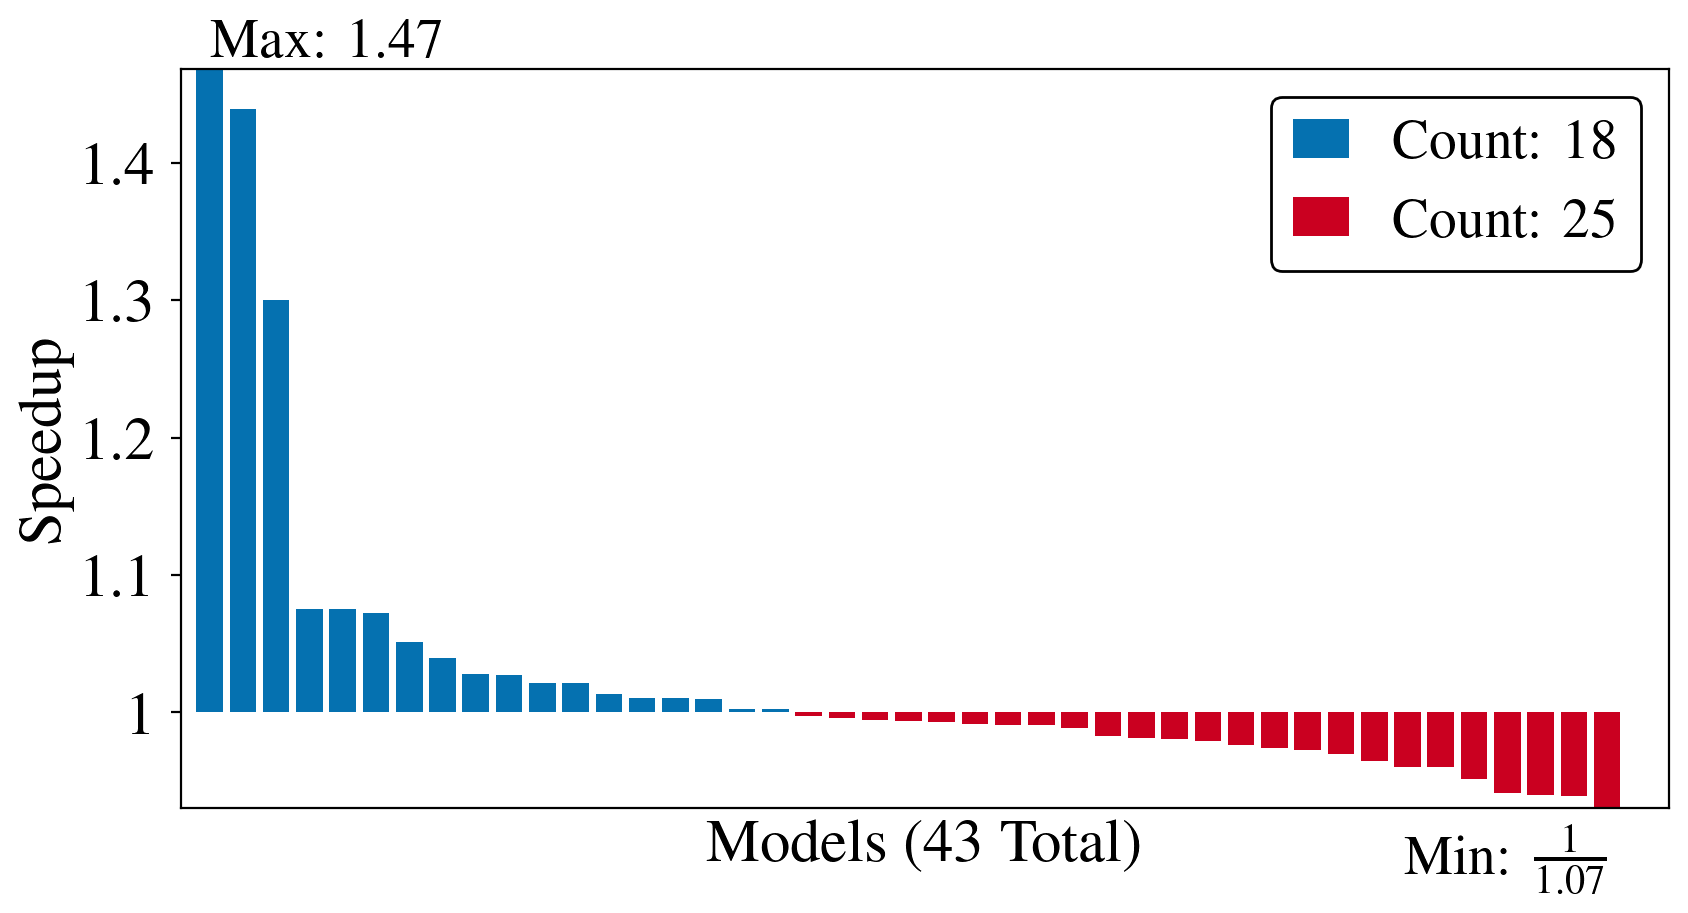
\includegraphics[width=\linewidth]{figures/end-to-end-torch-multithread.png}
        \caption{TorchVision, multi-thread}
        \label{fig:torch-multi}
    \end{subfigure}
    \begin{subfigure}{\columnwidth}
        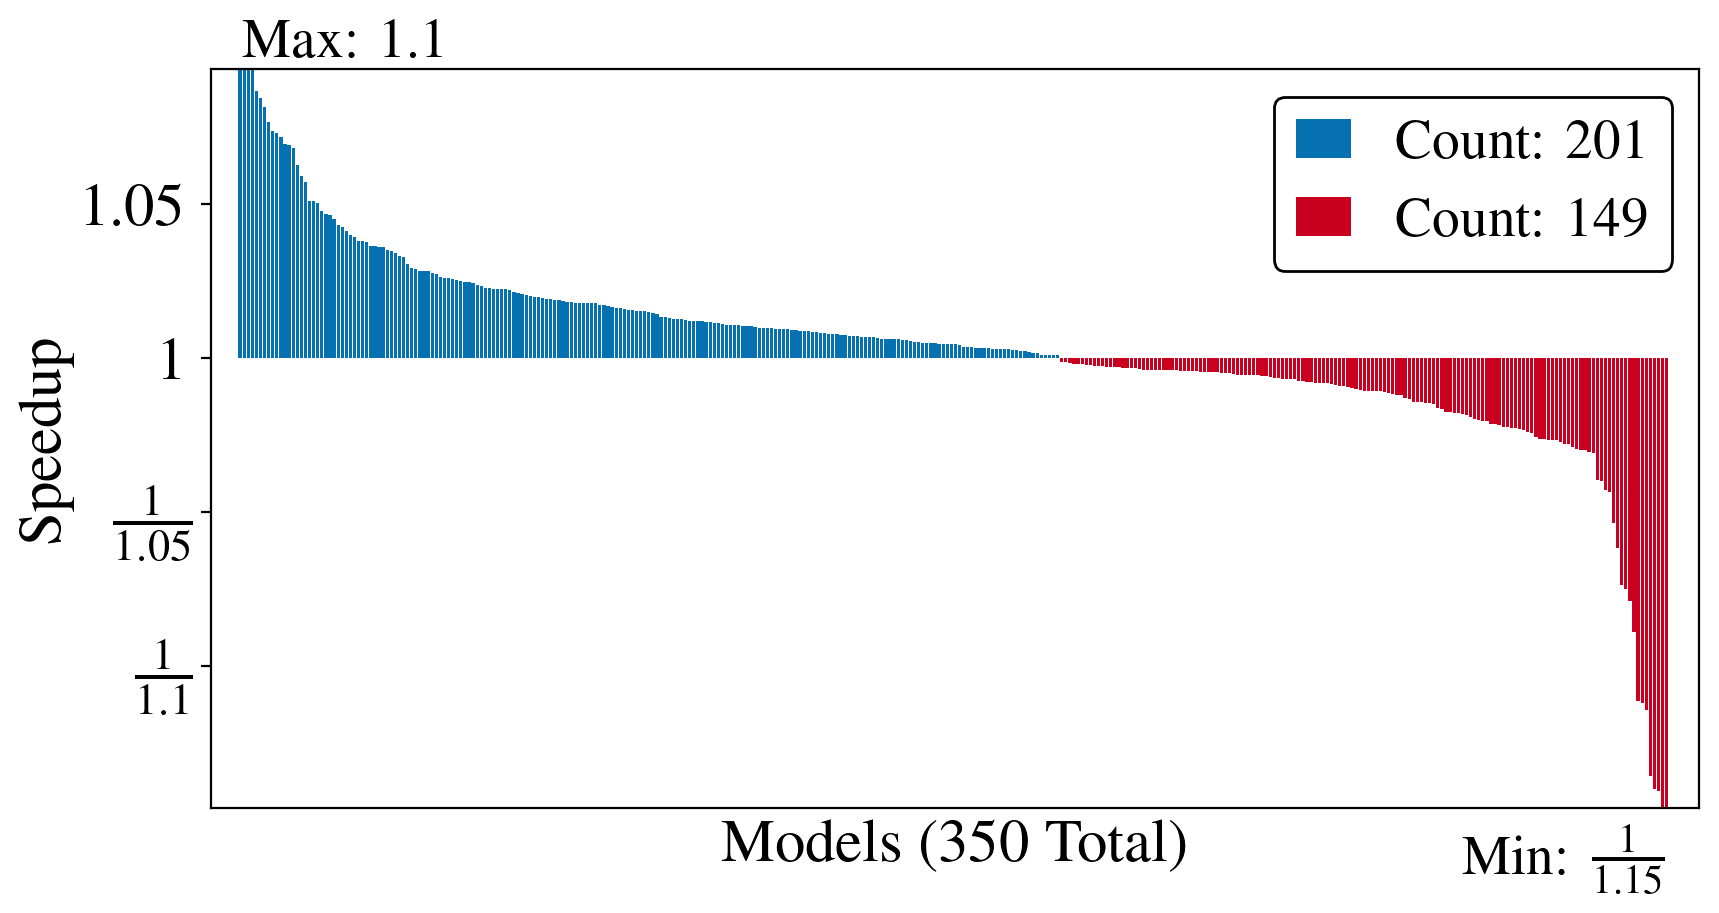
\includegraphics[width=\linewidth]{figures/end-to-end-timm-multithread.png}
        \caption{Timm, multi-thread}
        \label{fig:timm-multi}
    \end{subfigure}
    \caption{Improvement of \textbf{PyTorch-\algname} over PyTorch on end-to-end models.}
    \label{fig:end-to-end-comparison}
\end{figure}


Figures \ref{fig:timm-multi} and \ref{fig:torch-multi} compare PyTorch-\algname against PyTorch across Timm and TorchVision models for multithreaded execution. 
Notably, the speedup ranges vary between graphs, with wider ranges present in the TorchVision results.
Overall, the speedup trends are less pronounced than in \rsec{standalone-conv} due to additional operations present in these models, and the fact that not all convolutional layers utilize \algname.
Across all results, the highest observed speedup is 1.47$\times$, while the largest slowdown is 1.15$\times$.
The impact of \algname on performance depends on the specific combination of convolutional layers present in each model.
